\documentclass[11pt,a4paper]{article}

% ---------- Packages ----------
\usepackage[utf8]{inputenc}
\usepackage[T1]{fontenc}
% \usepackage{lmodern}  % optional, improves font rendering if installed
\usepackage[margin=1in]{geometry}
\usepackage{amsmath,amssymb,amsthm}
\usepackage{graphicx}
\usepackage{float}
\usepackage{booktabs}
\usepackage{hyperref}
\usepackage{url}
\usepackage{doi}
\usepackage[numbers,sort&compress]{natbib}
\usepackage{xcolor}
\usepackage{authblk}
\usepackage{tikz}
\usepackage{float}

\usetikzlibrary{arrows.meta, positioning, fit, backgrounds, calc}

\hypersetup{
  colorlinks=true,
  linkcolor=blue!60!black,
  citecolor=blue!60!black,
  urlcolor=blue!60!black
}

\newtheorem{proposition}{Proposition}

% ---------- Title ----------
\title{\textbf{Learning Travel-Time Embeddings\\
for Real-Time Isochrone Queries}}

\author{Mathias Vandaele}
\affil{Independent Research\\ \texttt{mathias.vandaele@pm.me}}

\date{April 2026}

\begin{document}
\maketitle

% ---------- Abstract ----------
\begin{abstract}
Computing travel times between addresses traditionally requires graph
routing engines such as OSRM or Valhalla, whose per-query latency makes
interactive applications --- real-time isochrones, dense clustering,
spatial joins over millions of points --- prohibitive. We present a
learned continuous representation of $\sim$33~million French addresses
in which the Euclidean distance between two embedding vectors directly
approximates their driving time. A single-tower network maps
$(\text{lat},\text{lon})$ through a Space2Vec multi-scale Fourier
encoding, a small residual backbone with GELU pre-activations, and a
linear projection into $\mathbb{R}^{64}$; we show that this linear head
induces a learned Mahalanobis metric in backbone feature space. Trained
against $\approx$432~million OSRM-supervised pairs with a pure $\ell_1$
loss, the model reaches a mean absolute error of \textbf{1.40~minutes}
(Spearman $\rho = 0.9989$), with $96.8\%$ of predictions within five
minutes of ground truth. A custom vector database, RingDB, answers
\emph{ring} queries
$\{v : d_\text{min} < \|q - v\| < d_\text{max}\}$ over the full corpus
via a SIMD-vectorized brute-force scan that exploits pre-cached
squared norms, saturates the machine's memory bandwidth on commodity
hardware, and outperforms a pivot-based pruning index we also tried.
We discuss why, the surprising empirical finding that the embedding
space spontaneously recovers France's road topology without ever
seeing map data, and the negative result that made us abandon
hyperbolic geometry for this task.
\end{abstract}

% =====================================================================
\section{Introduction}
% =====================================================================

Interactive mapping applications ask a simple question at enormous
scale: ``which places are reachable from here in less than $T$
minutes?'' Answering this well requires driving times, not
straight-line distances, because real road networks are shaped by
highways, one-way streets, rivers, mountains, and urban density. The
canonical answer is to run a shortest-path query on a routing
graph~\cite{luxen2011osrm,valhalla}. For a single query this is fast;
for \emph{millions} of queries --- the workload behind live isochrones
on a slider, neighbourhood clustering, or dense spatial joins --- it
is not, and the engineering around precomputation, contraction
hierarchies, and tile caches dominates production systems.

This paper explores a different trade-off. We ask whether driving time
can be approximated well enough by a \emph{continuous} function of a
pair of coordinates that the routing graph can be replaced, at
inference time, by a small neural network plus a vector database.
Concretely, we want a mapping $f : \mathbb{R}^2 \to \mathbb{R}^d$ such
that
\begin{equation}
  \bigl\lVert f(x_1) - f(x_2) \bigr\rVert_2 \;\approx\; T(x_1, x_2),
  \label{eq:core}
\end{equation}
where $T$ denotes driving time. If such an $f$ exists with sufficient
accuracy, every question that used to require a routing engine
collapses into a metric-space operation: ``reachable in $T$ minutes''
becomes a ball query, ``closest reachable addresses'' becomes
$k$-nearest neighbours, ``the boundary of the reachable region''
becomes a ring query.

Our contributions are as follows.
\begin{enumerate}
  \item \textbf{A compact model for a country-scale metric.} A
    $\approx$10~M-parameter single-tower network encodes $\sim$33~M
    French addresses into $\mathbb{R}^{64}$ such that Euclidean
    distance matches OSRM travel time to $1.40$~minutes MAE on
    held-out pairs.
  \item \textbf{A geometric interpretation of the projection head.}
    The final linear layer $W \in \mathbb{R}^{64 \times 1024}$ is not
    an arbitrary bottleneck: we prove that it induces a learned
    Mahalanobis metric $M = W^\top W$ of rank at most 64 in the
    backbone's 1024-dimensional feature space. This explains why a
    purely linear head is sufficient and why further non-linearity
    there would be redundant with the backbone.
  \item \textbf{RingDB: brute-force ring queries done right.} Instead
    of returning a full ball or a $k$-NN list, RingDB returns exactly
    the points in the annular shell
    $\{v : d_\text{min} < \|q - v\| < d_\text{max}\}$, which is the
    natural primitive for isochrone frontiers. Rather than pruning
    with pivots (which we tried and abandoned), RingDB pre-caches
    every vector's squared norm and reduces the entire query to one
    GEMV plus an elementwise test via the identity
    $\|a-b\|^2 = \|a\|^2 + \|b\|^2 - 2\langle a,b\rangle$. On
    commodity laptop hardware this approaches the machine's memory
    bandwidth ceiling.
  \item \textbf{A negative result on hyperbolic geometry.} An earlier
    version of this work used Poincar\'e-ball embeddings, motivated
    by the intuition that road networks are hierarchical. We report
    in detail why this failed --- learnable-curvature experiments
    let the model itself vote against the ball --- and why Euclidean
    space with a learned Mahalanobis metric is a better fit for a
    road \emph{mesh}.
  \item \textbf{Emergent topology.} A UMAP projection of the learned
    embeddings reveals that the model has spontaneously reconstructed
    the French road network --- highway filaments, geographically
    isolated clusters, physical barriers such as rivers and rail
    lines --- despite never having seen a map. Travel-time supervision
    alone is sufficient to recover topology.
\end{enumerate}

% =====================================================================
\section{Related Work}
% =====================================================================

\paragraph{Graph-based routing.}
Production routing engines such as OSRM~\cite{luxen2011osrm} and
Valhalla~\cite{valhalla} implement contraction hierarchies and
multi-level Dijkstra variants over OpenStreetMap. They answer single
queries in milliseconds but scale badly to workloads that demand many
simultaneous reachability computations; approximate alternatives such
as time-dependent contraction hierarchies still need the graph in
memory.

\paragraph{Learned ETA.}
Recent work at production scale has used graph neural networks and
sequence models to predict estimated times of arrival conditional on
a given route~\cite{derrow2021eta}. These models assume the route
already exists and focus on traffic-aware adjustment. Our setting is
different: we want the pairwise time between \emph{arbitrary} origins
and destinations, without ever materializing a route.

\paragraph{Metric embeddings.}
Learning embeddings such that a simple distance approximates a costly
target function is a classical idea in information retrieval and
metric learning~\cite{hadsell2006dimensionality,schroff2015facenet}.
The closest cousin to our approach is work that learns Euclidean
embeddings of graph nodes so that shortest-path distances can be
approximated by a simple vector operation~\cite{rizi2018shortest},
but that line of work operates on the nodes of a fixed, given graph
--- typically a social network --- and does not ingest raw geographic
coordinates. We want the opposite: a model that takes
$(\text{lat}, \text{lon})$ in and produces an embedding out, with no
graph ever materialised at inference time.

\paragraph{Coordinate encodings.}
Fourier feature encodings from NeRF~\cite{tancik2020fourier} and
Space2Vec~\cite{mai2020space2vec} have become the default way to feed
low-dimensional continuous positions into MLPs. We use the Space2Vec
variant --- log-spaced wavelengths covering five orders of geographic
scale, combined with random unit directions --- as the input block
of our network.

\paragraph{Hyperbolic representations.}
Poincar\'e-ball embeddings excel at tree-like
hierarchies~\cite{nickel2017poincare,ganea2018hyperbolic}. Early in
this project we conjectured that road networks, with Paris as a root
and departments as branches, would benefit from such geometry. Our
Section~\ref{sec:negative} reports why this intuition is wrong for
driving times: real road networks are \emph{meshes}, not trees, and
hyperbolic space collapses everything to the ball's boundary.

% =====================================================================
\section{Method}
\label{sec:method}
% =====================================================================

\subsection{Overall architecture}
The network is a single tower that maps a pair of geographic
coordinates to a vector in $\mathbb{R}^{64}$:
\[
  (\text{lat}, \text{lon}) \;\longrightarrow\;
  \text{xyz} \;\longrightarrow\;
  \underbrace{\phi(\cdot)}_{\text{Space2Vec}} \;\longrightarrow\;
  \underbrace{g(\cdot)}_{\text{residual backbone}} \;\longrightarrow\;
  \underbrace{W \cdot (\cdot) + b_W}_{\text{linear head}}
  \;\longrightarrow\; z \in \mathbb{R}^{64}.
\]
Since it is a single tower, the induced metric is symmetric by
construction: $\|f(A) - f(B)\| = \|f(B) - f(A)\|$. An earlier
dual-tower variant was explored to capture asymmetries caused by
one-way streets and elevation, but on the static, daytime-averaged
OSRM labels used here the symmetric tower matches it in accuracy and
is simpler to deploy. Total trainable parameters: $10{,}057{,}281$
(backbone $9{,}974{,}784$; projection head $65{,}600$; mapping MLP
$16{,}897$; Space2Vec buffer frozen).
Figure~\ref{fig:architecture} shows the full pipeline.

\begin{figure}[H]
\centering
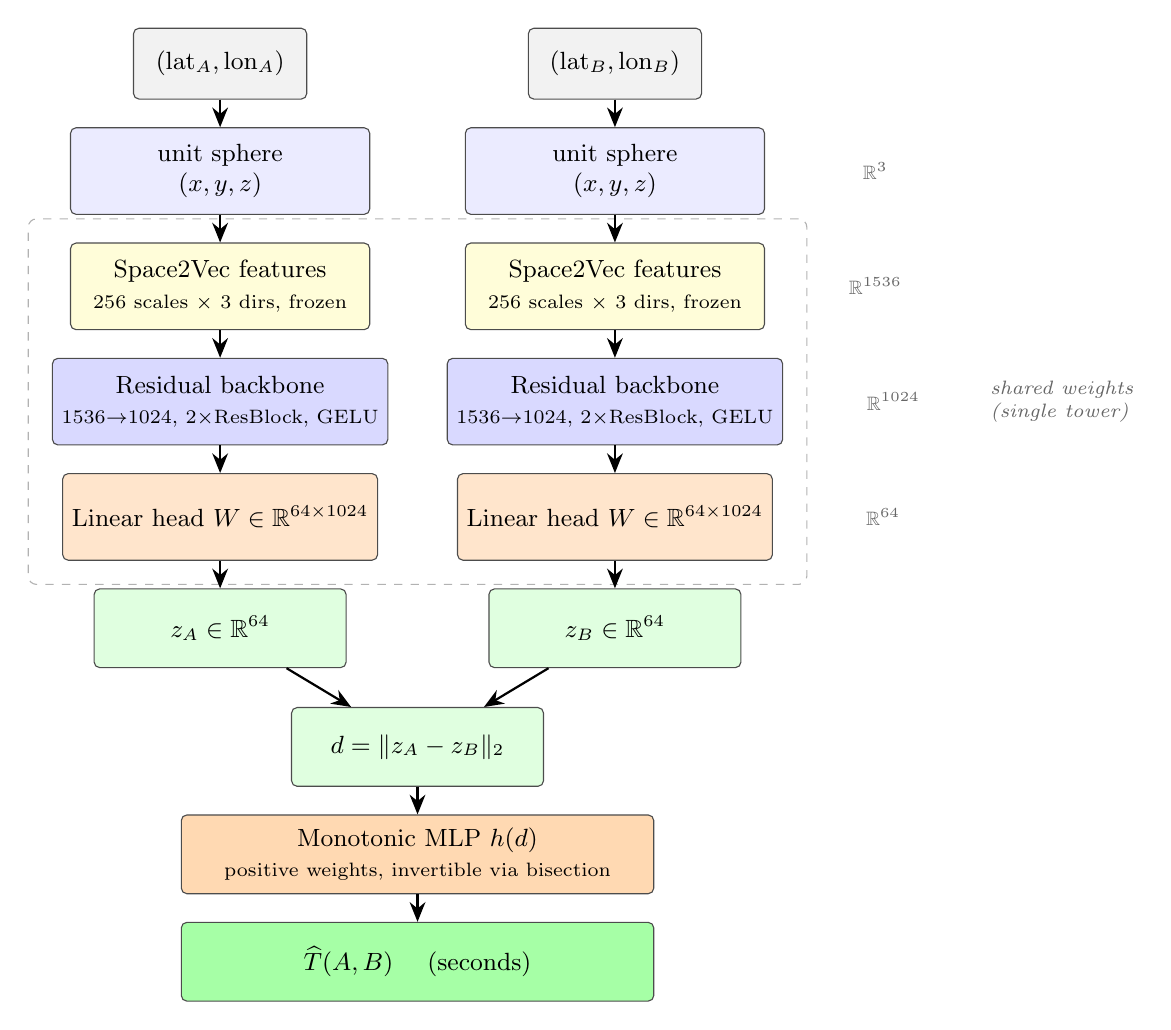
\begin{tikzpicture}[
    >={Stealth[length=2.5mm,width=2mm]},
    font=\small,
    node distance=3.5mm and 6mm,
    input/.style   = {rectangle, rounded corners=2pt, draw=black!70,
                      fill=gray!10, minimum width=22mm, minimum height=9mm,
                      align=center, font=\small},
    block/.style   = {rectangle, rounded corners=2pt, draw=black!70,
                      fill=blue!8,  minimum width=38mm, minimum height=11mm,
                      align=center, font=\small},
    backbone/.style= {rectangle, rounded corners=2pt, draw=black!70,
                      fill=blue!15, minimum width=38mm, minimum height=11mm,
                      align=center, font=\small},
    head/.style    = {rectangle, rounded corners=2pt, draw=black!70,
                      fill=orange!20, minimum width=38mm, minimum height=11mm,
                      align=center, font=\small},
    dist/.style    = {rectangle, rounded corners=2pt, draw=black!70,
                      fill=green!12, minimum width=32mm, minimum height=10mm,
                      align=center, font=\small},
    output/.style  = {rectangle, rounded corners=2pt, draw=black!70,
                      fill=green!25, minimum width=32mm, minimum height=10mm,
                      align=center, font=\small},
    dims/.style    = {font=\scriptsize\itshape, text=black!60},
]

\node[input] (latlonA) {$(\mathrm{lat}_A,\mathrm{lon}_A)$};
\node[input, right=28mm of latlonA] (latlonB) {$(\mathrm{lat}_B,\mathrm{lon}_B)$};

\node[block, below=of latlonA]  (xyzA) {unit sphere \\ $(x,y,z)$};
\node[block, below=of latlonB]  (xyzB) {unit sphere \\ $(x,y,z)$};

\node[block, fill=yellow!15, below=of xyzA, minimum width=38mm] (s2vA)
    {Space2Vec features \\ {\scriptsize 256 scales $\times$ 3 dirs, frozen}};
\node[block, fill=yellow!15, below=of xyzB, minimum width=38mm] (s2vB)
    {Space2Vec features \\ {\scriptsize 256 scales $\times$ 3 dirs, frozen}};

\node[backbone, below=of s2vA] (bbA)
    {Residual backbone \\ {\scriptsize 1536$\to$1024, 2$\times$ResBlock, GELU}};
\node[backbone, below=of s2vB] (bbB)
    {Residual backbone \\ {\scriptsize 1536$\to$1024, 2$\times$ResBlock, GELU}};

\node[head, below=of bbA] (headA)
    {Linear head $W \in \mathbb{R}^{64\times 1024}$};
\node[head, below=of bbB] (headB)
    {Linear head $W \in \mathbb{R}^{64\times 1024}$};

\node[dist, below=of headA] (embA) {$z_A \in \mathbb{R}^{64}$};
\node[dist, below=of headB] (embB) {$z_B \in \mathbb{R}^{64}$};

\node[dist, below=10mm of $(embA)!0.5!(embB)$] (l2)
    {$d = \|z_A - z_B\|_2$};

\node[output, below=of l2, fill=orange!30, minimum width=60mm] (mono)
    {Monotonic MLP $h(d)$ \\ {\scriptsize positive weights, invertible via bisection}};

\node[output, below=of mono, fill=green!35, minimum width=60mm] (time)
    {$\widehat{T}(A,B)$ \quad (seconds)};

\draw[->, thick] (latlonA) -- (xyzA);
\draw[->, thick] (latlonB) -- (xyzB);
\draw[->, thick] (xyzA)    -- (s2vA);
\draw[->, thick] (xyzB)    -- (s2vB);
\draw[->, thick] (s2vA)    -- (bbA);
\draw[->, thick] (s2vB)    -- (bbB);
\draw[->, thick] (bbA)     -- (headA);
\draw[->, thick] (bbB)     -- (headB);
\draw[->, thick] (headA)   -- (embA);
\draw[->, thick] (headB)   -- (embB);
\draw[->, thick] (embA)    -- (l2);
\draw[->, thick] (embB)    -- (l2);
\draw[->, thick] (l2)      -- (mono);
\draw[->, thick] (mono)    -- (time);

\begin{pgfonlayer}{background}
  \node[draw=black!30, dashed, rounded corners=3pt,
        inner sep=3mm,
        fit=(s2vA)(s2vB)(bbA)(bbB)(headA)(headB)] (tower) {};
\end{pgfonlayer}
\node[anchor=west, font=\scriptsize\itshape, text=black!60, align=left]
  at ([xshift=22mm]tower.east)
  {shared weights \\ (single tower)};

\node[dims] at ([xshift=14mm]xyzB.east)  {$\mathbb{R}^{3}$};
\node[dims] at ([xshift=14mm]s2vB.east)  {$\mathbb{R}^{1536}$};
\node[dims] at ([xshift=14mm]bbB.east)   {$\mathbb{R}^{1024}$};
\node[dims] at ([xshift=14mm]headB.east) {$\mathbb{R}^{64}$};

\end{tikzpicture}
\caption{The pipeline. Two addresses $A$ and $B$ are independently
encoded by a \emph{single} shared tower --- Space2Vec multi-scale
Fourier features, a residual backbone, and a linear projection head
into $\mathbb{R}^{64}$ --- and their embeddings are compared by
Euclidean distance. A monotonic MLP then maps this distance to a
predicted travel time in seconds. Because the mapping is monotone, it
is invertible by bisection, which turns isochrone queries ``reachable
in $T$ minutes'' into ring queries in embedding space. The linear
head $W$ induces a learned Mahalanobis metric $M = W^{\top}W$ of rank
at most $64$ in the backbone's $1024$-dimensional feature space
(Proposition~\ref{prop:maha}).}
\label{fig:architecture}
\end{figure}

\subsection{Input: unit-sphere coordinates (no centering)}
Latitude and longitude are mapped to unit-sphere coordinates
$(x, y, z) = (\cos\phi\cos\lambda, \cos\phi\sin\lambda, \sin\phi)$ to
remove the longitudinal compression of planar projections. No
recentering or rescaling is applied. Naively, one might worry that
metropolitan France occupies only $\sim$$0.04\%$ of the unit sphere,
giving Fourier features too narrow an input range; Space2Vec's
multi-scale wavelengths (below) handle this directly by placing basis
functions at every geographically relevant scale, so the raw
unit-sphere coordinates are sufficient.

\subsection{Space2Vec Fourier features}
We use a multi-scale Fourier encoding in the style of
Space2Vec~\cite{mai2020space2vec}. We choose $S = 256$ wavelengths
log-spaced from $\lambda_{\min} = 10$~m to
$\lambda_{\max} = 1000$~km,
\[
  \lambda_s \;=\; \lambda_{\min}
  \cdot \bigl(\lambda_{\max}/\lambda_{\min}\bigr)^{s/(S-1)},
  \qquad s = 0,\ldots,S-1,
\]
covering five orders of geographic scale, from city-block granularity
to country-level structure. For each scale $s$ we draw three random
unit directions
$\hat b_{s,1}, \hat b_{s,2}, \hat b_{s,3} \in \mathbb{R}^{3}$
and form frequency vectors
$b_{s,j} = \hat b_{s,j} \cdot (R_\oplus / \lambda_s)$, where $R_\oplus$
is the Earth radius. With this scaling, a geodesic of length
$\lambda_s$ advances the argument of $b_{s,j}^{\top} x$ by $2\pi$,
which is exactly what ``a wavelength'' means at the corresponding
spatial scale. Stacking all $3S = 768$ frequency vectors as columns
of a matrix $B \in \mathbb{R}^{3 \times 768}$, the features are
\[
  \phi(x) \;=\;
  \bigl[\,\sin(2\pi\, B^{\top} x),\;\cos(2\pi\, B^{\top} x)\,\bigr]
  \in \mathbb{R}^{1536}.
\]
The matrix $B$ is stored as a non-trainable buffer. This resolves the
dynamic-range problem without any input centering or rescaling: each
wavelength contributes features tuned to its own geographic scale,
and the model sees block-level, city-level, regional, and
country-level structure from the first layer onward.

\subsection{Residual backbone}
The backbone $g$ is a small residual MLP. An input projection takes
$\mathbb{R}^{1536}$ to $\mathbb{R}^{1024}$, followed by two
pre-activation residual blocks and a final LayerNorm. Each block
implements
\[
  x \;\mapsto\; x \;+\; L_2\!\bigl(\,\text{GELU}\bigl(L_1(\text{GELU}(\text{LN}(x)))\bigr)\,\bigr),
\]
with a $2\times$ expansion ($1024 \to 2048 \to 1024$). The backbone
has $9{,}974{,}784$ parameters and is by far the largest component.
The width of 1024 is deliberately chosen to be much larger than the
output dimension: the backbone is an over-parameterized feature space
that the linear head will then \emph{select from}.

\subsection{The linear projection head as a learned Mahalanobis metric}
\label{sec:mahalanobis}
The final layer is a single projection
$W \in \mathbb{R}^{64 \times 1024}$ with bias $b_W$,
\[
  f(x) \;=\; W\, g(\phi(x)) \;+\; b_W.
\]
The squared Euclidean distance between two embeddings is bias-free
(the bias cancels in the difference) and factors cleanly:
\begin{align}
  \|f(A) - f(B)\|_{2}^{\,2}
  &= \bigl\| W\,(g(A) - g(B)) \bigr\|_{2}^{\,2} \nonumber\\
  &= \bigl(g(A) - g(B)\bigr)^{\!\top}\!
     \underbrace{W^{\!\top} W}_{=:\,M}\,
     \bigl(g(A) - g(B)\bigr). \label{eq:maha}
\end{align}

\begin{proposition}
\label{prop:maha}
The matrix $M = W^{\top} W \in \mathbb{R}^{1024 \times 1024}$ is
symmetric positive semi-definite with $\mathrm{rank}(M) \leq 64$.
The squared embedding distance \eqref{eq:maha} is therefore a
\emph{Mahalanobis pseudo-distance} in the 1024-dimensional backbone
feature space, with precision matrix $M$.
\end{proposition}

\begin{proof}
Symmetry: $M^{\top} = (W^{\top} W)^{\top} = W^{\top} W$. For any
$v$, $v^{\top} M v = \|Wv\|_{2}^{2} \geq 0$, so $M$ is PSD.
Finally, $\mathrm{rank}(M) = \mathrm{rank}(W^{\top} W)
= \mathrm{rank}(W) \leq 64$. The bilinear form~\eqref{eq:maha}
therefore has the algebraic signature of a Mahalanobis metric,
degenerate on $\ker(W)$. \qed
\end{proof}

This observation has three practical consequences.

\emph{(i) Why a linear head is enough.} A metric is a bilinear form;
linear projection composed with $\ell_{2}$ is exactly that form. Any
further non-linearity in the head would \emph{not} give us a
different metric structure, only a different non-linear embedding
--- which the backbone can already express. The head is not an
arbitrary bottleneck; it is the minimal functional form capable of
producing a metric.

\emph{(ii) What the model actually learns.} A rank-64 projection of
a 1024-dimensional feature space picks out the 64 most
travel-time-discriminative directions in backbone space. Directions
orthogonal to $\operatorname{range}(W^{\top})$ are explicitly
ignored: the model says ``these variations in the backbone's
representation do not matter for travel time.'' The backbone is
allowed to be rich and redundant; the head is what disciplines it.

\emph{(iii) Low effective dimensionality is predicted, not a bug.}
Empirically, the 64-dimensional embedding space has an intrinsic
dimension of $\approx$9.9 (Section~\ref{sec:results}). Rather than
treating this as ``wasted capacity,'' Proposition~\ref{prop:maha}
explains it: road-network travel times lie on a low-dimensional
manifold, and the Mahalanobis metric discovers that dimensionality
on its own. We return to this in Section~\ref{sec:ringdb}, where it
matters for the vector index.

\subsection{From distance to seconds: a monotonic mapping MLP}
The relationship between Euclidean distance in embedding space and
travel time in seconds is monotonic but not linear: short urban trips
and long inter-regional trips live in different regimes, and no
two-parameter formula (linear, log, power, tanh) fits both well. We
therefore use a small \emph{monotonic} MLP
$h : \mathbb{R}_{\geq 0} \to \mathbb{R}_{\geq 0}$ with three layers
of width 128 and positive-weight reparameterization:
\[
  h(d) \;=\; \mathrm{softplus}\!\Bigl(\,W_{3}^{+}\,
    \mathrm{ReLU}\bigl(W_{2}^{+}\,
      \mathrm{ReLU}(W_{1}^{+} d + b_{1})
    + b_{2}\bigr) + b_{3}\Bigr),
\]
where each weight matrix
$W_{i}^{+} = \mathrm{softplus}(\widetilde W_{i})$ is elementwise
non-negative. Positive-weight monotone networks have a long history
going back at least to Sill's min-max networks and the analysis of
Daniels and Velikova~\cite{daniels2010monotone}; more recent work by
Wehenkel and Louppe~\cite{wehenkel2019umnn} establishes that the
positive-weight construction remains a universal approximator of
monotone functions when composed with suitable activations. The
composition of non-negative linear maps, ReLUs, and a final softplus
is non-decreasing, which matters for two reasons:

\begin{itemize}
  \item The prediction $\hat T = h(\|f(A) - f(B)\|)$ is automatically
    monotone in embedding distance, ruling out pathological solutions
    where nearby embeddings are predicted to be far in time.
  \item $h$ is easily inverted by bisection in $\approx$20 iterations
    (cost $< 0.01$~ms). Isochrone queries --- ``addresses within
    $T$ minutes'' --- are converted into ring queries by computing
    $h^{-1}(T \pm \varepsilon)$ once per request.
\end{itemize}
The mapping MLP has $16{,}897$ parameters and is optimized jointly
with everything else, with a $2\times$ learning-rate multiplier.

% =====================================================================
\section{Training}
\label{sec:training}
% =====================================================================

\subsection{Dataset: 432~M OSRM-supervised pairs}
Training pairs are generated from the French \emph{Base Adresses
Nationale} (BAN), which lists $\approx$33~M addressable points across
metropolitan France. For each pair of addresses $(A, B)$ we query OSRM
with the default car profile for the driving time $T(A, B)$ in
seconds. We generated $\approx$469.5~M raw pairs on a 112-thread AMD
EPYC instance over seven hours on spot pricing (total cloud cost:
\$9); after removing overseas territories (poor OSM coverage) and
near-zero trivial pairs, $431{,}789{,}950$ records remain. The
empirical time distribution is log-normal, with median 65~min and a
tail reaching $\sim$14~h for cross-country trips.

We hold out 1~M pairs from the end of the shuffled Parquet file for
validation and use the remaining $\approx$430~M for streaming training.

\subsection{Loss}
We minimise a pure $\ell_{1}$ loss on predicted seconds:
\[
  \mathcal{L} \;=\; \frac{1}{N} \sum_{i=1}^{N}
  \bigl|\,\hat T_{i} - T_{i}\,\bigr|,
  \qquad
  \hat T_{i} = h\!\bigl(\|f(A_{i}) - f(B_{i})\|_{2}\bigr).
\]
Earlier variants used log-space MSE (to equalise relative error
across scales) and smooth-$\ell_{1}$; pure $\ell_{1}$ gave uniformly
better per-bucket MAE in our setting, likely because it neither
under-penalizes long trips (as log-space MSE does) nor introduces a
quadratic region near zero that biases the optimizer toward many
small corrections instead of the large corrections the model
actually needs in early training.

\subsection{Optimisation}
We train with AdamW, initial learning rate $10^{-3}$ (with a
$2\times$ multiplier for the mapping MLP), weight decay $10^{-5}$,
cosine annealing schedule with $\eta_{\min} = 10^{-6}$, batch size
8192, mixed precision (AMP) on a single NVIDIA GPU. Gradient clipping
is set to $\|g\|\leq 5$. Ten epochs over the full 432~M dataset take
$\approx$6~hours on an L4-class GPU; each epoch is
$\approx$52{,}586 batches, with one validation pass per epoch.

% =====================================================================
\section{Results}
\label{sec:results}
% =====================================================================

\subsection{Accuracy}
Table~\ref{tab:headline} reports headline metrics on 1~M held-out
validation pairs after ten epochs. Mean absolute error is
1.40~minutes overall, with Spearman correlation $\rho = 0.9989$,
meaning the induced ordering of reachable destinations is essentially
perfect.

\begin{table}[h]
\centering
\caption{Headline validation metrics after 10 epochs on 1~M held-out pairs.}
\label{tab:headline}
\begin{tabular}{lr}
\toprule
Metric & Value \\
\midrule
MAE (minutes)                     & \textbf{1.40} \\
MAE (seconds)                     & 84 \\
Pearson $r$                       & 0.9659 \\
Spearman $\rho$                   & \textbf{0.9989} \\
Predictions within 1 minute       & 52.8\% \\
Predictions within 2 minutes      & 77.6\% \\
Predictions within 5 minutes      & 96.8\% \\
Predictions within 10 minutes     & 99.7\% \\
MAPE (trips $>$ 5 min)            & 3.9\% \\
Median relative error             & 1.5\% \\
\bottomrule
\end{tabular}
\end{table}

Table~\ref{tab:buckets} breaks this down by trip duration. Error
scales sub-linearly: a 0--10~min trip has median error
$\approx$0.6~min ($\approx$36~s), while a 4~h+ trip has median error
1.5~min despite being on the order of 240~minutes long. This is the
behaviour a log-normal error model would predict, but achieved here
with a pure $\ell_{1}$ loss.

\begin{table}[h]
\centering
\caption{Per-bucket validation MAE at the best epoch.}
\label{tab:buckets}
\begin{tabular}{lrrrr}
\toprule
Bucket & MAE (min) & Median (min) & P90 (min) & \# pairs \\
\midrule
0--10~min  & 0.8 & 0.6 & 1.7 & 35{,}317 \\
10--30~min & 1.4 & 1.0 & 3.0 & 26{,}809 \\
30--60~min & 1.4 & 1.0 & 3.0 & 31{,}894 \\
1--2~h     & 1.4 & 1.0 & 3.0 & 58{,}124 \\
2--4~h     & 1.8 & 1.1 & 4.1 & 34{,}925 \\
4~h+       & 2.3 & 1.5 & 5.4 & 12{,}931 \\
\bottomrule
\end{tabular}
\end{table}

\subsection{Embedding geometry and intrinsic dimension}
After training, embeddings have norm $31.2 \pm 1.2$ and mean pairwise
L2 distance $\approx$7.05. A PCA on the validation embeddings shows
that 24 components explain 90\% of the variance and 57 explain 99\%;
the participation-ratio effective dimension is $\approx$9.9. Rather
than a symptom of under-utilisation, this is \emph{consistent} with
Proposition~\ref{prop:maha}: the Mahalanobis metric $M = W^{\top} W$
has rank at most 64, and the observed effective dimension reflects
the intrinsic dimensionality of the travel-time manifold itself,
which is much smaller than the nominal 64 available.

\subsection{Emergent road topology}
Projecting the 64-dimensional embeddings to 2D via UMAP reveals,
without any geographic supervision, the structure of the French road
network (Figure~\ref{fig:umap}): major roads appear as thin
filaments, cities cluster by commune, and travel-time barriers are
visible as gaps and discontinuities between clusters.

\begin{figure}[H]
\centering
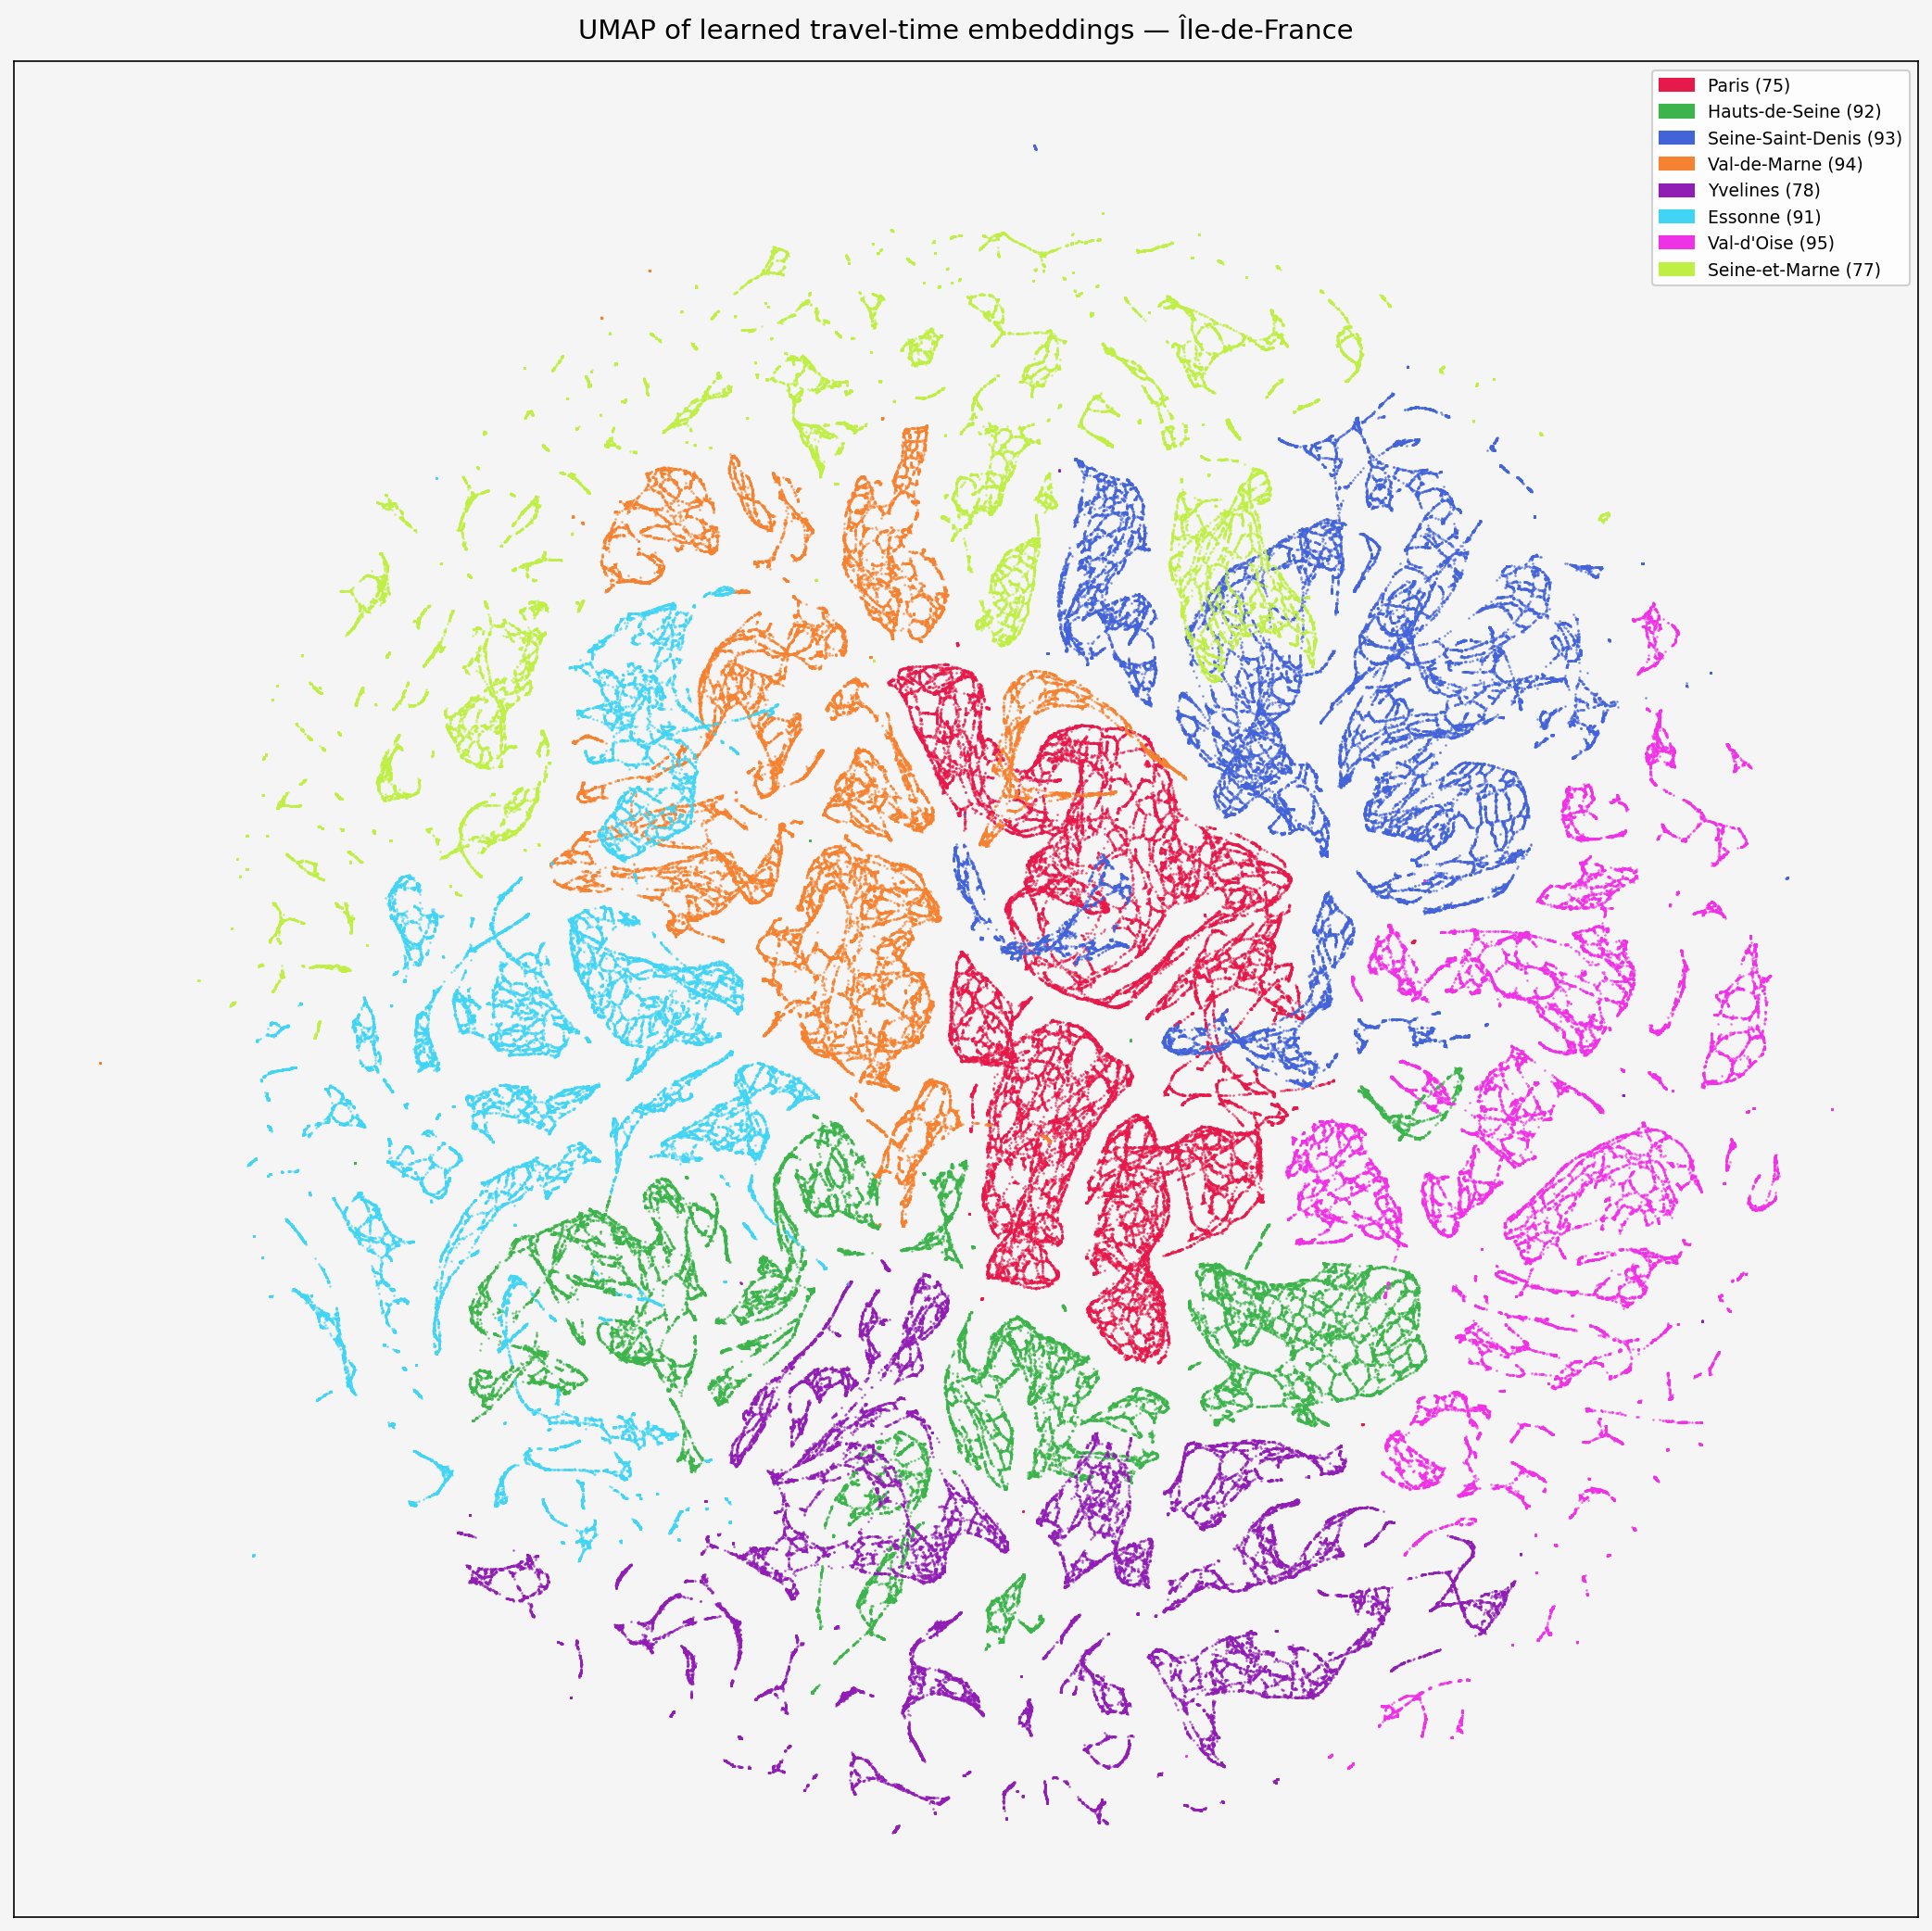
\includegraphics[width=1.0\linewidth]{umap_idf.png}
\caption{UMAP projection of learned 64-dimensional embeddings for
addresses in \^{I}le-de-France, coloured by d\'{e}partement.
Paris (75, red) sits at the centre; the inner-ring d\'{e}partements
--- Hauts-de-Seine (92), Seine-Saint-Denis (93), Val-de-Marne (94)
--- form a tight cluster around it; the outer d\'{e}partements
--- Yvelines (78), Essonne (91), Val-d'Oise (95), Seine-et-Marne (77)
--- occupy the periphery.
This concentric structure mirrors the actual geography of the
Paris ring roads (P\'{e}riph\'{e}rique, A86, Francilienne) and was
never provided to the model: it emerges purely from travel-time
supervision.
Within each d\'{e}partement, filament structures correspond to
individual road segments and branching points to junctions.
Administrative boundaries are respected without ever appearing
in the training signal.}
\label{fig:umap}
\end{figure}

% =====================================================================
\section{RingDB: Brute-Force Ring Queries via Cached Norms}
\label{sec:ringdb}
% =====================================================================

Accurate embeddings are only half of the story; production
applications demand fast spatial queries over the full $\sim$33~M
address corpus. We built RingDB~\cite{ringdb}, a specialised vector
database whose primary query is not $k$-nearest neighbours but the
annular \emph{ring}:
\begin{equation}
  \mathrm{Ring}(q, d_\text{min}, d_\text{max}) \;=\;
  \bigl\{\,v \in V \;\mid\; d_\text{min} \,<\, \|q - v\|_{2} \,<\, d_\text{max}\,\bigr\}.
  \label{eq:ring}
\end{equation}
RingDB returns exactly the frontier of an isochrone without ever
materialising its interior.

\subsection{Why rings, not balls}
Isochrone rendering does not need every address inside the reachable
region --- only the boundary. A contour in the plane is determined by
its frontier points; interior points are redundant. Choosing
$d_\text{min} = h^{-1}(T - \varepsilon)$ and
$d_\text{max} = h^{-1}(T + \varepsilon)$ returns only the
$\sim$5000~addresses lying on the edge of the ``$T$-minutes
reachable'' region. Crucially, this keeps the result-set size roughly
\emph{constant} as the underlying corpus grows, which is what makes
constant-latency isochrones possible.

\subsection{The expansion identity}
The design of RingDB turns on a single elementary observation. For
any two vectors $a, b \in \mathbb{R}^{d}$,
\begin{equation}
  \|a - b\|_{2}^{\,2}
  \;=\; (a - b) \cdot (a - b)
  \;=\; \|a\|_{2}^{\,2} \;+\; \|b\|_{2}^{\,2}
  \;-\; 2\,\langle a, b\rangle.
  \label{eq:expansion}
\end{equation}
If $\|v\|_{2}^{\,2}$ is precomputed and cached for every database
vector, and $\|q\|_{2}^{\,2}$ is computed once per query, then the
only per-vector work needed to evaluate $\|q - v\|_{2}^{\,2}$ is one
inner product $\langle q, v\rangle$. Collecting all $N$ database
vectors as the rows of a matrix
$D \in \mathbb{R}^{N \times d}$, the vector of inner products across
the entire corpus is a single matrix--vector product,
$D\,q \in \mathbb{R}^{N}$, and the full set of pairwise squared
distances is
\[
  \mathrm{sq\_dists}
  \;=\; \underbrace{\|q\|_{2}^{\,2}\,\mathbf{1}}_{\text{scalar broadcast}}
  \;+\; \underbrace{n_{v}}_{\text{cached vector in } \mathbb{R}^{N}}
  \;-\; 2\,(D\,q),
\]
where $n_{v} \in \mathbb{R}^{N}$ is the cached squared-norm column.
The ring test~\eqref{eq:ring} then reduces to a single elementwise
comparison against
$[d_\text{min}^{\,2},\,d_\text{max}^{\,2}]$.

This turns the entire query into one GEMV (general matrix--vector
product) plus an elementwise pass over a vector of length $N$. Both
operations are perfectly sequential in memory, SIMD-friendly, and
memory-bandwidth bound --- the best-case workload for any modern CPU
or GPU. In practice the implementation fuses the two operations into
a single streaming pass over the rows of $D$ (Section~\ref{sec:impl})
so that the intermediate $Dq$ vector is never materialised; the fused
version is what the latency numbers below refer to.

\subsection{What we tried before this, and why it failed}
Our first design was a pivot-based index using the triangle
inequality in the style of classical metric trees. A small set of
$k$-means centroids served as pivots; for each data point we stored
its distance to every pivot, and at query time we used the triangle
inequality to bound $\|q - v\|$ and prune candidates without ever
loading their coordinates. On paper this looked like a clean win:
real embeddings have low intrinsic dimension ($\approx$9.9), which
is exactly the regime where pivot pruning is supposed to shine.

In practice, \emph{almost nothing got pruned}. The embedding
distribution is geometrically tight --- norms $31.2 \pm 1.2$, mean
pairwise distance $\approx$7 --- so triangle-inequality bounds rarely
excluded candidates with high confidence, and the per-candidate
overhead of bitmap lookups and bound evaluations was not cheap
enough to amortise against the few candidates that \emph{were}
eliminated. The end-to-end query time was consistently worse than a
straightforward brute-force scan.

The brute-force scan via~\eqref{eq:expansion} has two decisive
advantages that pivot methods struggle to match:

\begin{enumerate}
  \item \textbf{No per-candidate branching.} Every database point is
    touched in the same way, via fused multiply--adds in a tight
    dot-product loop. There is no cache-hostile random access, no
    bitmap intersection, no bound evaluation. The inner loop is a
    dense reduction whose SIMD instruction mix has been a compiler
    target for decades and which a modern CPU can essentially run at
    memory-bandwidth speed.
  \item \textbf{Pre-cached norms convert a quadratic problem into a
    linear one.} Without caching, $\|q - v\|^{2}$ would require
    reading both $q$ and $v$, subtracting, and re-squaring per
    candidate. With cached $\|v\|^{2}$, only the dot product
    $\langle q, v\rangle$ is computed per candidate, and the rest is
    scalar arithmetic. The memory traffic becomes essentially
    $O(N \cdot d)$ (a single streaming read of $D$) plus $O(N)$ (a
    streaming read of cached norms), which is close to the minimum
    any algorithm could achieve for this problem.
\end{enumerate}

\subsection{Implementation}
\label{sec:impl}
RingDB is implemented in Rust~\cite{ringdb}. The on-disk layout is a
handful of memory-mapped flat binary files: \texttt{meta.bin} records
the pair $(\text{dims}, N)$ as two little-endian \texttt{u64} values;
\texttt{vectors.bin} holds the matrix $D$ as row-major \texttt{f32}
($N \cdot d$ floats, $\approx$7.9~GB for $N = 33$~M at $d = 64$);
\texttt{norms\_sq.bin} holds the pre-computed squared norms
$\|v_i\|_{2}^{\,2}$ as a contiguous \texttt{f32} column
($\approx$130~MB); and \texttt{payloads.bin} plus \texttt{offsets.bin}
store per-vector metadata (addresses, lat/lon, external IDs). All
files are opened once via \texttt{mmap} and accessed as typed slices,
so there is no deserialisation cost and no per-query allocation.

The core query primitive is a single parallel pass over the rows of
$D$. For each row $v_{i}$ the loop body computes one dot product
$\langle q, v_{i} \rangle$, reconstructs $\|q - v_{i}\|_{2}^{\,2}$
from the cached norms via equation~\eqref{eq:expansion}, and tests
the result against $[d_{\min}^{\,2}, d_{\max}^{\,2}]$. A disk (ball)
query is the same loop with only the upper bound checked; both
primitives share the same scan code and differ only in a single
constant-time comparison.

The dot product itself is a hand-written Rust routine with
\emph{four independent} floating-point accumulators fed by fused
multiply--adds (\texttt{f32::mul\_add}). Breaking the reduction into
four parallel partial sums removes the loop-carried dependency that
would otherwise bottleneck a naive dot product on FMA latency, which
is essential for reaching peak floating-point throughput on modern
pipelined FPUs. Combined with \texttt{chunks\_exact(4)} over the
input slices, this pattern is one that LLVM reliably auto-vectorises
into \texttt{fmla.4s} on ARM NEON and \texttt{vfmadd} on x86 AVX;
we verified the generated assembly with \texttt{cargo asm} to
confirm that the intended SIMD instructions are actually emitted,
and not replaced by a scalar fallback or broken up by the optimiser.
No BLAS dependency is required: the compiler-emitted kernels match
a hand-tuned GEMV closely enough that the additional integration
cost would be wasted.

Parallelism across rows is handled by Rayon's
\texttt{par\_chunks\_exact}: the scan is embarrassingly parallel
along $N$, each worker thread owns a contiguous slab of the
memory-mapped matrix, and the surviving candidates are gathered
into the result via a standard parallel \texttt{filter\_map}. The
result type is a plain \texttt{\#[repr(C)]} struct holding the
vector index and squared distance --- a \emph{plain old datum} that
can be memcopied and streamed over a wire without serialisation.

\subsection{Measured performance}
On a single Apple M3 Pro laptop, the exact brute-force scan over
30~M 64-dimensional vectors runs at $\approx$67~ms. This is within
a small constant of the theoretical memory bandwidth ceiling of the
machine: the scan is bandwidth-bound, not compute-bound, which
means additional optimisation effort on the arithmetic side would
be wasted. The full isochrone pipeline --- embed the query address,
invert $h$ to obtain $(d_\text{min}, d_\text{max})$, run the ring
scan, compute an alpha shape over the $\sim$5000 returned frontier
points, serialise a GeoJSON polygon --- completes well inside the
16~ms budget for 60\,fps on modest server hardware, and in tens of
milliseconds on the laptop. A GPU backend via CUDA is in progress
and is projected to bring the scan to $\sim$8~ms on an RTX-class
GPU through the same dot-product-plus-mask recipe.

% =====================================================================
\section{Applications}
% =====================================================================

The combination of an accurate metric and a ring index unlocks a
small family of interactive applications that are awkward or
impossible on top of a conventional routing engine.

\paragraph{A motivating example.}
Consider a real-estate search with compound reachability constraints:
``show me apartments within 25 minutes of Gare de Lyon, within
45 minutes of Charles de Gaulle airport, and within one hour of
Disneyland Paris.'' In the routing-engine framing this is a cross
product of three shortest-path computations per candidate, over tens
of millions of candidates --- effectively impossible interactively,
and cache-hostile at any scale. In our framing, each reachability
constraint is a single disk query in embedding space (the same
primitive RingDB uses for rings, with only the upper bound checked);
the three result sets are intersected by ID; and the entire query,
over the full 33~M-address corpus, completes in well under half a
second on the laptop. The compound version of the question is not
just \emph{faster} than the routing-engine version --- it is
\emph{practically new}, in the sense that no end user would ever
have considered asking it of a routing API. That is what we mean
when we say the metric embedding unlocks applications rather than
merely accelerating them.

\paragraph{Real-time isochrones.}
A slider that controls ``$T$ minutes from here'' becomes trivial:
each drag event issues a ring query for the new $T$, runs a morphing
concave hull on the $\sim$5000 returned frontier points, and streams
the resulting polygon to a web client over WebSocket. Because the
result-set size does not grow with $T$, latency is constant in the
slider position.

\begin{figure}[H]
\centering
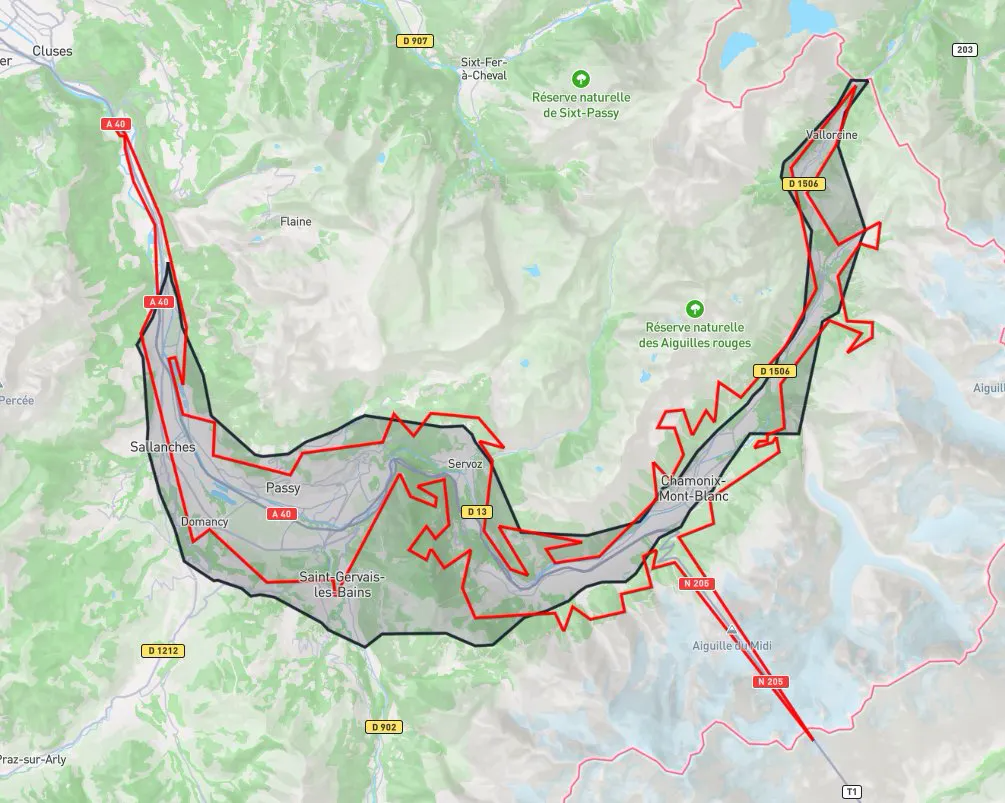
\includegraphics[width=1.0\linewidth]{chamonix_isochrone.png}
\caption{45-minute driving isochrone centred on the Chamonix valley.
\textbf{Black}: our system (ring query + alpha-shape contour).
\textbf{Red}: OSRM ground truth.
The valley crescent is correctly recovered despite the model never
having seen map data during training.
Differences arise from two expected sources: highway segments
(A40, N205) are absent from the BAN address corpus and therefore
produce no frontier points, eliminating the ground-truth spikes;
and our contour smooths over micro-topology artifacts
--- switchbacks, dead-end mountain roads --- that cause the
OSRM polygon to be non-convex in ways that would be
misleading on a rendered map layer.
The Chamonix valley is a deliberate stress test: vertical
Alpine walls and a single access corridor make this one of the
most constrained isochrone geometries in metropolitan France.}
\label{fig:chamonix}
\end{figure}

\paragraph{Spatial clustering on travel time.}
Clustering addresses by driving-time similarity rather than
straight-line distance is a natural request for logistics and
location intelligence, and is intractable with a routing backend.
In our embedding space it is a standard $k$-means or HDBSCAN over
the 64-dimensional vectors.

\paragraph{Reachability joins for real estate.}
Listings can be filtered by compound constraints such as ``within
25~minutes of a school, 40~minutes of an office, and 1~hour of an
airport'' by intersecting three ball queries in embedding space ---
a primitive RingDB supports directly by replacing the lower bound
with zero.

\paragraph{Travel-time Voronoi diagrams.}
Given a set of points of interest, partitioning the map by
closest-in-time POI becomes a single vector-index pass.

% =====================================================================
\section{The Negative Result: Why Not Hyperbolic Space?}
\label{sec:negative}
% =====================================================================

An earlier generation of this work embedded addresses into the
Poincar\'e ball rather than Euclidean space. The intuition was
seductive: road networks look hierarchical (Paris as a root,
departments as branches), and hyperbolic space is famously efficient
for trees~\cite{nickel2017poincare}. We abandoned the approach after
extensive experimentation because it failed in an instructive way.

With a fixed ball of curvature $c = 1$, embeddings systematically
collapsed to the ball's boundary: $\|f(x)\| \to 1$ with standard
deviation $\to 0$ across the dataset. Replacing the soft projection
with a hard clamp at $0.9$ simply produced collapse at $0.9$. Adding
a learnable curvature parameter let the model itself vote: $c$
drifted from $0.1$ to $6.57$, i.e., the network chose to
\emph{shrink} the ball so that radius $R = 1/\sqrt{c}$ became tiny,
which is mathematically equivalent to destroying the hyperbolic
structure. On comparable 10~M-pair experiments, Euclidean embeddings
reached $\approx$14.5~min MAE while the best Poincar\'e variant
stalled at $\approx$14.9~min with degenerate boundary norms.

The diagnosis we settled on is that \emph{France's road network is
a mesh, not a tree}. Lille--Strasbourg, Lyon--Marseille,
Bordeaux--Toulouse are all \emph{direct} connections that do not
route through any central hub. Mesh metric spaces need uniform
capacity at all scales, which Euclidean (and a Mahalanobis metric
over Euclidean) provides and which the hyperbolic ball does not: in
$d$ dimensions the hyperbolic volume element scales as
$\sinh^{d-1}(r)$, so almost all representational capacity is
concentrated in a vanishing shell near the boundary, and gradient
descent pushes everything there. The learnable-curvature experiment
is, in retrospect, the cleanest possible evidence: given the option,
the model itself votes against the ball.

Figure~\ref{fig:curvature} visualises this trajectory on the 10~M-pair
experiment. Initialised at $c = 0.1$ (a Poincar\'e ball of radius
$R = 1/\sqrt{c} \approx 3.16$), gradient descent steadily pushes
$c$ upward to $6.57$ over twenty epochs, shrinking the ball's radius
to $R \approx 0.39$. Throughout, the embedding-norm standard
deviation stays pinned at zero: \emph{every} embedding sits on the
boundary regardless of where that boundary is. The model is not
finding a better ball; it is trying to destroy the one it was given.

\begin{figure}[H]
\centering
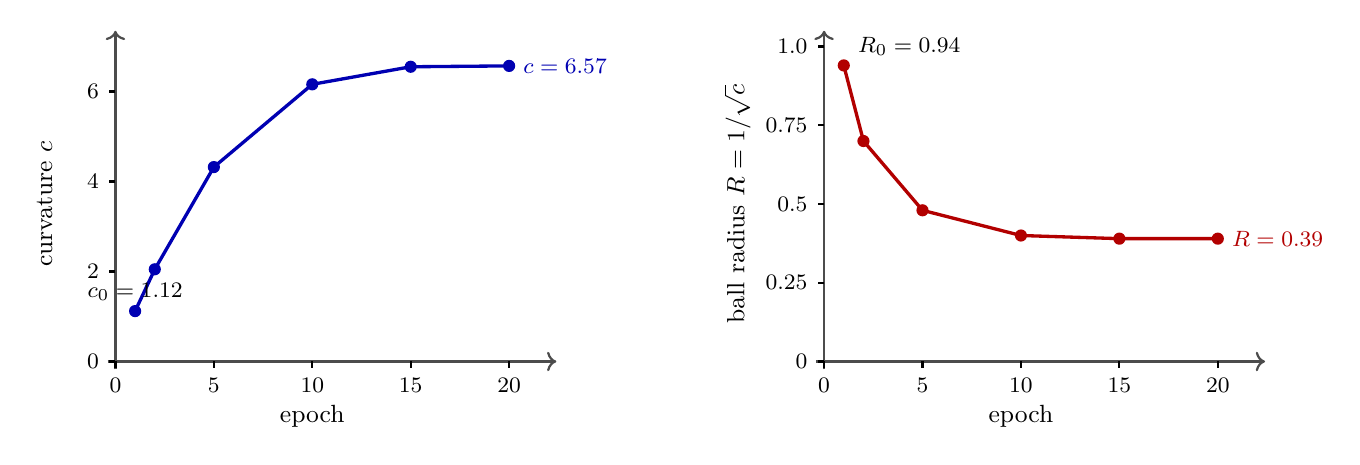
\begin{tikzpicture}[thick]
  % ---- Left subplot: curvature c(epoch) ----
  \begin{scope}
    \draw[->, black!70] (-0.1,0) -- (5.6,0);
    \draw[->, black!70] (0,-0.1) -- (0,4.2);
    \node[font=\small] at (2.5,-0.7) {epoch};
    \node[rotate=90, font=\small] at (-0.9,2) {curvature $c$};
    % X ticks: epoch 0, 5, 10, 15, 20 → x = 0, 1.25, 2.5, 3.75, 5
    \foreach \x/\l in {0/0, 1.25/5, 2.5/10, 3.75/15, 5/20}
      \draw (\x,0) -- (\x,-0.08) node[below, font=\footnotesize] {\l};
    % Y ticks: c = 0, 2, 4, 6 → y = 0, 1.143, 2.286, 3.429 (scale y = c * 4/7)
    \foreach \y/\l in {0/0, 1.143/2, 2.286/4, 3.429/6}
      \draw (0,\y) -- (-0.08,\y) node[left, font=\footnotesize] {\l};
    % Data line: (epoch, c) → (x, y) with x = epoch*0.25, y = c * 4/7
    \draw[blue!70!black, very thick]
      (0.25,0.640) -- (0.50,1.171) -- (1.25,2.469) -- (2.50,3.520)
      -- (3.75,3.743) -- (5.00,3.754);
    \foreach \x/\y in {0.25/0.640, 0.50/1.171, 1.25/2.469,
                       2.50/3.520, 3.75/3.743, 5.00/3.754}
      \fill[blue!70!black] (\x,\y) circle (2.2pt);
    \node[blue!70!black, font=\footnotesize, right] at (5.05, 3.75) {$c = 6.57$};
    \node[font=\footnotesize, above] at (0.25, 0.640) {$c_0 = 1.12$};
  \end{scope}

  % ---- Right subplot: ball radius R(epoch) ----
  \begin{scope}[shift={(9,0)}]
    \draw[->, black!70] (-0.1,0) -- (5.6,0);
    \draw[->, black!70] (0,-0.1) -- (0,4.2);
    \node[font=\small] at (2.5,-0.7) {epoch};
    \node[rotate=90, font=\small] at (-1.1,2) {ball radius $R = 1/\sqrt{c}$};
    % X ticks: same as left
    \foreach \x/\l in {0/0, 1.25/5, 2.5/10, 3.75/15, 5/20}
      \draw (\x,0) -- (\x,-0.08) node[below, font=\footnotesize] {\l};
    % Y ticks: R = 0, 0.25, 0.5, 0.75, 1.0 → y = 0, 1, 2, 3, 4
    \foreach \y/\l in {0/0, 1/0.25, 2/0.5, 3/0.75, 4/1.0}
      \draw (0,\y) -- (-0.08,\y) node[left, font=\footnotesize] {\l};
    % Data line: (epoch, R) → (x, y) with x = epoch*0.25, y = R*4
    \draw[red!70!black, very thick]
      (0.25,3.76) -- (0.50,2.80) -- (1.25,1.92) -- (2.50,1.60)
      -- (3.75,1.56) -- (5.00,1.56);
    \foreach \x/\y in {0.25/3.76, 0.50/2.80, 1.25/1.92,
                       2.50/1.60, 3.75/1.56, 5.00/1.56}
      \fill[red!70!black] (\x,\y) circle (2.2pt);
    \node[red!70!black, font=\footnotesize, right] at (5.05, 1.56) {$R = 0.39$};
    \node[font=\footnotesize, above right] at (0.3, 3.76) {$R_0 = 0.94$};
  \end{scope}
\end{tikzpicture}
\caption{The learnable-curvature experiment on 10~M pairs. When the
Poincar\'e-ball curvature parameter $c$ is made trainable, gradient
descent steadily increases it (left), which is equivalent to
shrinking the ball's radius $R = 1/\sqrt{c}$ (right). Throughout the
whole run, the embedding-norm standard deviation remains pinned at
zero: every address sits exactly on the ball's boundary, regardless
of where the boundary is. Given the option, the network prefers to
shrink the ball toward a point rather than use its interior ---
which is the cleanest possible evidence that the hyperbolic geometry
is the wrong prior for this task.}
\label{fig:curvature}
\end{figure}

% =====================================================================
\section{Discussion and Limitations}
% =====================================================================

\paragraph{What the model is not.}
The reported metric approximates \emph{static, daytime-average} OSRM
times. It has no notion of live traffic, time of day, weather, road
closures, or vehicle class. For production ETA it would have to be
composed with a traffic-aware correction (which is the setting of
most learned-ETA literature); for the interactive applications we
target --- exploratory real estate search, logistics clustering,
reachability visualisation --- the static metric is usually exactly
what the user wants.

\paragraph{Error tails.}
The largest absolute errors consistently occur on a specific kind of
trip: medium-distance routes across geographic barriers (estuaries
in Brittany, the Rh\^one delta, the Alps). We read these as places
where OSRM itself takes an unusual detour that our smooth metric
cannot reproduce locally. A residual correction head conditioned on
per-route features could plausibly halve the tail, at the cost of
no longer being a pure metric.

\paragraph{Single tower vs. dual tower.}
We chose the symmetric single-tower model because, on the
daytime-average labels used here, a dual-tower asymmetric variant
offered no measurable gain. On labels that capture genuine asymmetry
(live rush-hour data, one-way-heavy historical centres) dual towers
would likely matter again. The loss of asymmetry is a deliberate
trade-off, not a limitation of the approach.

\paragraph{The pivot-pruning cautionary tale.}
We emphasise Section~\ref{sec:ringdb}'s failure because it is easy
to believe, in the abstract, that an index with a theoretically
favourable intrinsic-dimension profile \emph{must} outperform brute
force. In practice, on geometrically tight embedding distributions,
it does not: the savings from pruning are eaten alive by the
per-candidate overhead, and GEMV on cached norms wins by being the
simplest thing that saturates the memory bus. The lesson we draw is
that for sub-100~ms queries over tens of millions of
low-intrinsic-dim vectors, the right default is \emph{brute force
done well}, not a tree or pivot index that looks sophisticated on
paper.

\paragraph{Scaling to other countries.}
The entire pipeline is reproducible per country: an OSM extract, an
OSRM instance, a few days of spot-CPU time to generate pairs, and a
retraining run. The model's hyperparameters (Space2Vec wavelengths,
embedding dimension) are essentially country-agnostic.

% =====================================================================
\section{Conclusion}
% =====================================================================

We have shown that driving time over a country-scale road network
can be accurately represented as Euclidean distance in a learned
64-dimensional space, and that the machinery required to make this
useful --- a Space2Vec front-end, a small residual backbone, a
linear projection head that is in fact a learned Mahalanobis metric,
a monotonic invertible mapping to seconds, and a brute-force vector
database built around cached squared norms and the expansion
identity $\|a-b\|^{2} = \|a\|^{2} + \|b\|^{2} - 2\langle a,b\rangle$
--- fits comfortably on commodity hardware. On $\approx$432~million
OSRM pairs covering $\sim$33~M French addresses, the model reaches
1.40~min MAE and Spearman $\rho = 0.9989$, with $96.8\%$ of
predictions within five minutes of ground truth. The resulting
embedding space is not only accurate: it has spontaneously
reconstructed the topology of the French road network from
travel-time supervision alone. Along the way, the failure of
hyperbolic geometry on this task clarified what kind of metric
space road networks actually want --- a mesh, not a tree --- and
the failure of pivot-based pruning clarified how to build the
corresponding vector index: by doing nothing clever, as fast as the
memory bus allows.

\paragraph{Reproducibility.}
We intend to release a partial version of the training dataset, the
model architecture and training script, and the RingDB index code
under open licences. Full-corpus weights and the complete dataset
are retained for commercial reasons.

% ---------- References ----------
\bibliographystyle{plainnat}
\bibliography{references}

\end{document}